\documentclass[a4paper,12pt]{article}
\usepackage[utf8]{inputenc}
\usepackage{graphicx}
\usepackage{fancyhdr}
\usepackage{amsmath}
\usepackage{adjustbox}
\usepackage{mathtools}
\usepackage{float}
\usepackage[spanish, es-nodecimaldot]{babel} 
\usepackage{lastpage}
\usepackage{amssymb} % Para símbolos matemáticos adicionales
\usepackage{hyperref}
\usepackage{cleveref}
%\usepackage[none]{hyphenat}
\usepackage{array}

\usepackage{multirow}
\usepackage{textcomp}
\usepackage[left=2.5cm, right=2.5cm, top=3cm, bottom=3cm]{geometry}

\graphicspath{{Imagenes/}}

% Encabezado y pie de página
\pagestyle{fancy}
\fancyhf{}
\setlength{\headheight}{30 pt}
\renewcommand{\headrulewidth}{0.2pt}
\fancyhead[R]{\begin{tabular}{@{}l@{}}
\includegraphics[scale=0.4]{escudo.PNG}\end{tabular}}
\fancyhead[L]{\begin{tabular}{@{}c@{}} \textbf{Robótica I - Año: 2024} \\ Trabajo Práctico 4: Cinemática Directa \end{tabular}}


\fancyfoot[R]{\thepage}
\fancyfoot[C]{\begin{tabular}{@{}c@{}}\textbf{BORQUEZ PEREZ Juan Manuel}\\ \textbf{Legajo 13567}\end{tabular}}
\renewcommand{\footrulewidth}{0.2pt}

\begin{document}

\begin{titlepage}
    \centering
    \vspace*{5cm}
    {\Huge\bfseries Informe de Trabajo Práctico N°4}\\
    \vspace{0.2cm}
    {\Large \textbf{Cinemática Directa}}\\
    \vspace{0.5cm}
    {\Large Robótica I}\\
    \vspace{0.5 cm}
    {\Large Ingeniería en Mecatrónica}\\
    \vspace{0.2 cm}
    {\Large Facultad de Ingeniería - UNCUYO}\\
    \vspace{1.5cm}
    Alumno: Juan Manuel BORQUEZ PEREZ\\
    Legajo: 13567\\
    \vfill
    {\begin{tabular}{@{}c@{}}
\includegraphics[scale=0.4]{escudo.PNG}\end{tabular}}\hspace{10pt}
    %Año 2023
\end{titlepage}

\section{Ejercicio 1.}
\textbf{Trabaje en Matlab y resuelva la cinemática directa del Paint Mate 200iA (FANUC), para los siguientes arreglos de variables articulares}

\begin{figure}[H]
    \centering
    \begin{adjustbox}{scale = 0.35, max width=\columnwidth}
        \framebox{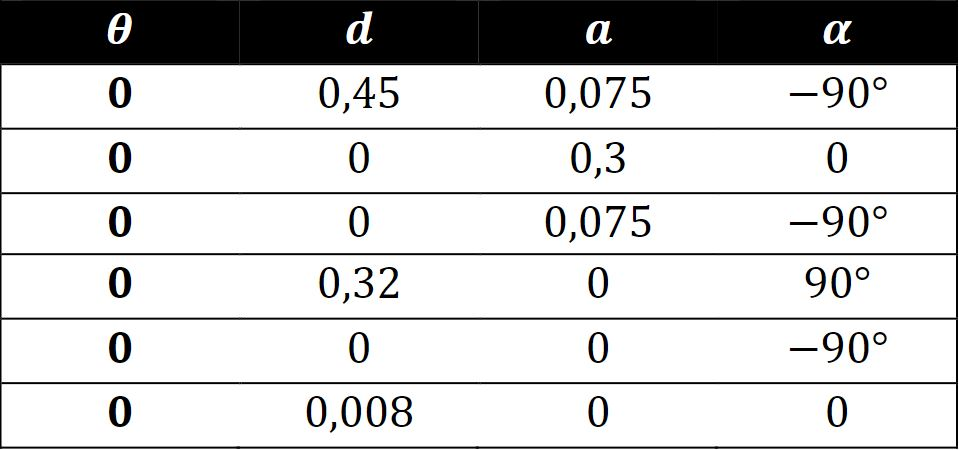
\includegraphics{1-DH_fanuc.JPG}}
    \end{adjustbox}
    \caption{Parametros DH Fanuc.}
\end{figure}

\subsection{}
Coordenadas articulares:
\begin{equation*}
    \overline{q}_1 = 
    \begin{bmatrix}
        0\,;0\,;0\,;0\,;0\,;0
    \end{bmatrix}
\end{equation*}

Matriz de transformación total:
\begin{equation}
    \left(\begin{array}{cccc} 1.0 & 0 & 0 & 0.45\\ 0 & -1.0 & 0 & 0\\ 0 & 0 & -1.0 & 0.122\\ 0 & 0 & 0 & 1.0 \end{array}\right)
    \label{T_q1}
\end{equation}

\subsection{}
Coordenadas articulares:
\begin{equation*}
    \overline{q}_2 = 
    \begin{bmatrix}
        \pi/4;-\pi/2\,\;0\,;0\,;0\,;0
    \end{bmatrix}
\end{equation*}

Matriz de transformación total:
\begin{equation}
    \left(\begin{array}{cccc} 0 & 0.7071 & 0.7071 & 0.285\\ 0 & -0.7071 & 0.7071 & 0.285\\ 1.0 & 0 & 0 & 0.825\\ 0 & 0 & 0 & 1.0 \end{array}\right)
    \label{T_q2}
\end{equation}

\subsection{}
Coordenadas articulares:
\begin{equation*}
    \overline{q}_3 = 
    \begin{bmatrix}
        \pi/5\,;-2\pi/5\,;-\pi/10\,;\pi/2\,;3\pi/10\,;-\pi/2
    \end{bmatrix}
\end{equation*}

Matriz de transformación total:
\begin{equation}
    \left(\begin{array}{cccc} 0 & 1.0 & 0 & 0.3946\\ 0 & 0 & 1.0 & 0.2947\\ 1.0 & 0 & 0 & 0.8103\\ 0 & 0 & 0 & 1.0 \end{array}\right)
    \label{T_q3}
\end{equation}

\subsection{}
Coordenadas articulares:
\begin{equation*}
    \overline{q}_4 = 
    \begin{bmatrix}
        -0.61\,;-0.15\,;-0.30\,;1.40\,;1.90\,;-1.40
    \end{bmatrix}
\end{equation*}

Matriz de transformación total:
\begin{equation}
    \left(\begin{array}{cccc} 0.8941 & 0.3322 & 0.3003 & 0.4764\\ -0.3545 & 0.1156 & 0.9279 & -0.3239\\ 0.2735 & -0.9361 & 0.2211 & 0.2411\\ 0 & 0 & 0 & 1.0 \end{array}\right)
    \label{T_q4}
\end{equation}

\begin{figure}[H]
    \centering
    \begin{adjustbox}{max width=\columnwidth}
        \framebox{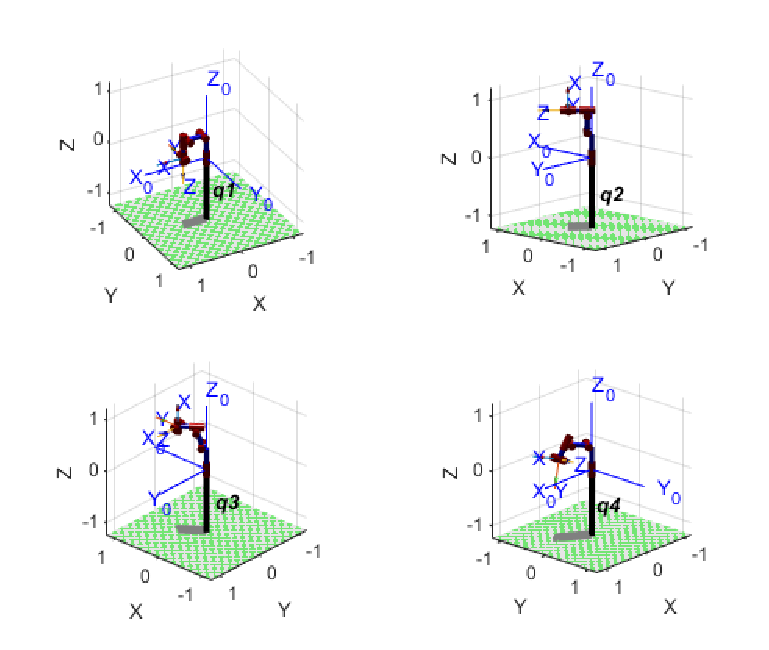
\includegraphics{2-Ejercicio_1_posiciones.pdf}}
    \end{adjustbox}
    \caption{Posiciones articulares correspondientes.}
\end{figure}

\section{Ejercicio 2.}
\subsection{Verificación del robot}
\label{subsec: verificacion}

Por observación de la matriz DH dada en comparación con la propuesta
en el TP3 para el mismo tipo de robot se puede identificar que se refieren
a distintos modelos. La que se confeccionó para el TP3 corresponde al 
SCARA IRB 910SC-3/0.45 mientras que la que se indica aquí corresponde al
SCARA IRB 910SC-3/0.55. La diferencia se presenta en el parámetro $L$ (\cref{diferencia SCARA}), que se corresponde
con el parámetro $a$ del $S_1$, en la fila 1 de la matrices DH (\cref{DH TP3} y \cref{DH TP4}). Además
se puede observar en la \cref{DH TP4} que los sistemas 2 y 1 coinciden en origen a lo largo del eje z
y también el sistema 4 comparte origen en el extremo final con el sistema 3, mientras que en \cref{DH TP3}
se tomó un desplazamiento en el eje z entre el sistema 1 y 2, y también entre el sistema 3 y 4.
Luego existe una diferencia en la medida tomada para la separación entre el sistema de la base
y el sistema 1.

\begin{figure}[H]
    \centering
    \begin{adjustbox}{scale = 0.85,max width=\columnwidth}
        \framebox{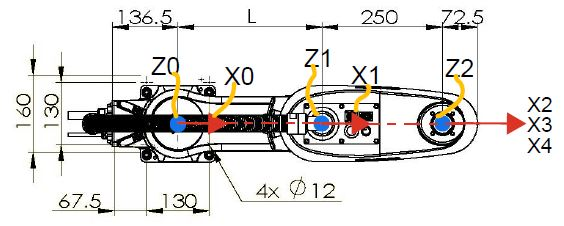
\includegraphics{3-SCARA_L.JPG}}
    \end{adjustbox}
    \caption{Indicación del parámetro L.}
    \label{diferencia SCARA}
\end{figure}

\begin{figure}[H]
    \centering
    \begin{adjustbox}{scale = 0.65, max width=\columnwidth}
        \framebox{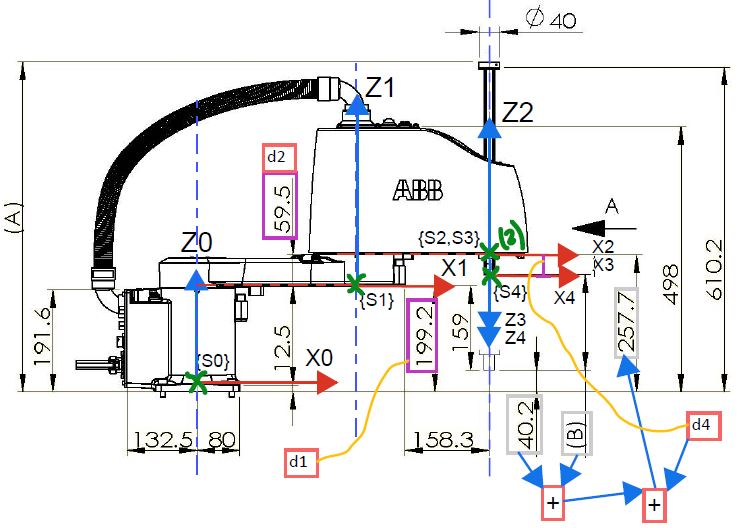
\includegraphics{4-SCARA_lateral.JPG}}
    \end{adjustbox}
    \caption{Vista lateral robot.}
    \label{vista lateral}
\end{figure}

\begin{table}[H]
    \centering
    \begin{tabular}{|c|c|c|c|c|c|}
    \hline
    Sistema & $\theta$  & $d$           & $a$      & $\alpha$ & $\sigma$ \\ \hline
    1       & $q_1$     & $0.1992$      & $0.200$  & 0.000    & 0        \\ \hline
    2       & $q_2$     & $0.0595$      & $0.250$  & 0.000    & 0        \\ \hline
    3       & $0.000$   & $q_3$         & $0.000$  & $\pi$      & 1        \\ \hline
    4       & $q_4$     & $0.0375$      & $0.000$  & 0.000    & 0        \\ \hline
    \end{tabular}
    \caption{Parámetros DH TP3.}
    \label{DH TP3}
\end{table}

\begin{table}[H]
    \centering
    \begin{tabular}{|c|c|c|c|c|c|}
    \hline
    Sistema & $\theta$  & $d$           & $a$      & $\alpha$ & $\sigma$ \\ \hline
    1       & $q_1$     & $0.195$       & $0.300$  & 0.000    & 0        \\ \hline
    2       & $q_2$     & $0.000$       & $0.250$  & 0.000    & 0        \\ \hline
    3       & $0.000$   & $q_3$         & $0.000$  & $\pi$      & 1        \\ \hline
    4       & $q_4$     & $0.000$       & $0.000$  & 0.000    & 0        \\ \hline
    \end{tabular}
    \caption{Parámetros DH TP4.}
    \label{DH TP4}
\end{table}

\begin{figure}[H]
    \centering
    \begin{adjustbox}{max width=\columnwidth}
        \framebox{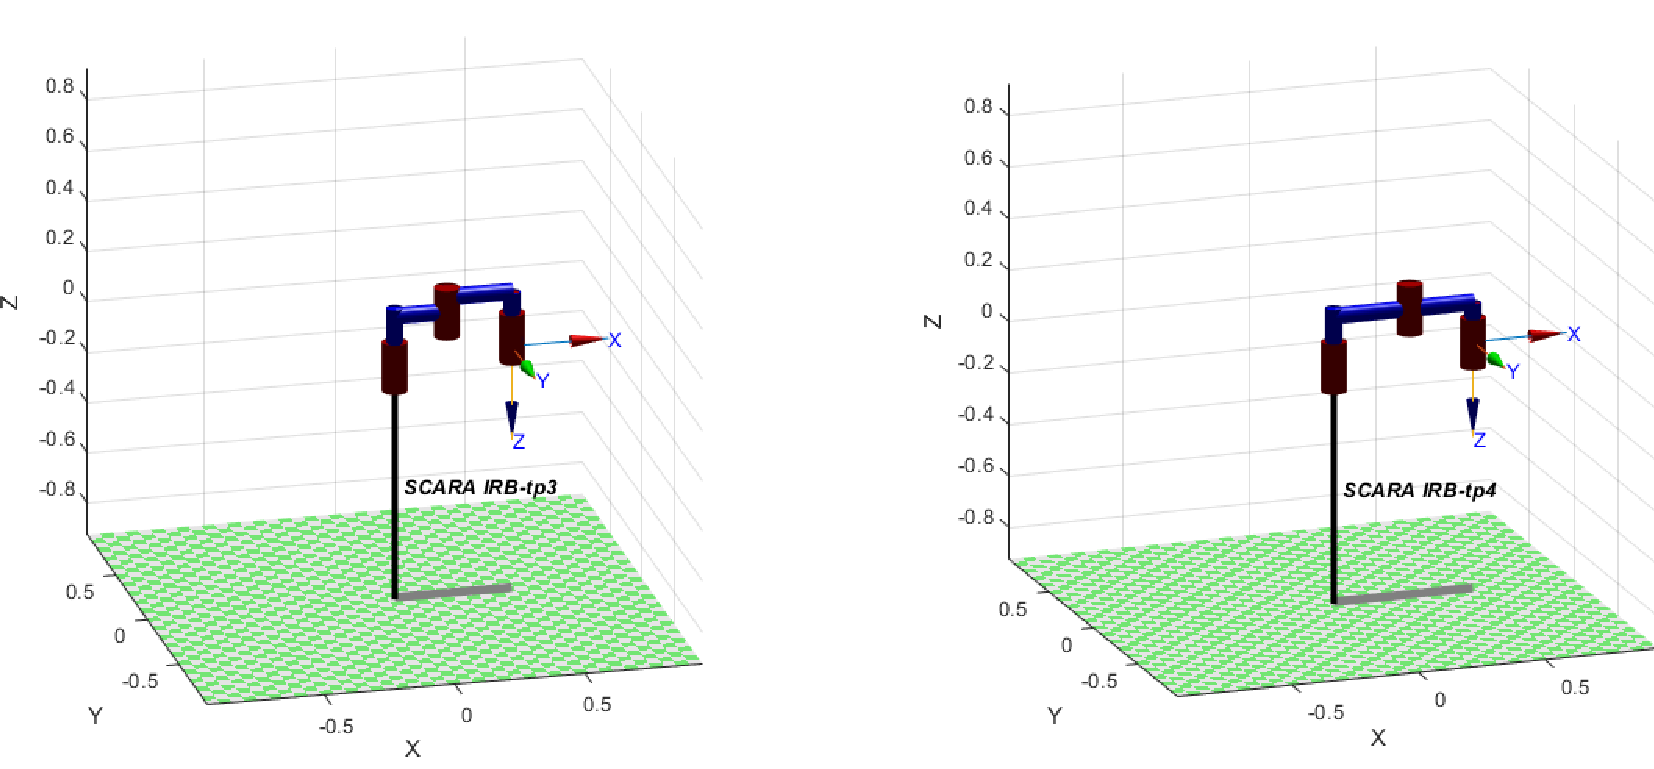
\includegraphics{4-Ejercicio_1_verificacion.pdf}}
    \end{adjustbox}
    \caption{Comparación de las definiciones.}
    \label{comparacion}
\end{figure}
En la anterior figura se comparan las definiciones. Considero que es mas eficiente la definición
dada en este TP en lugar de los desplazamientos de los sistemas como se presentó en el TP3.


\begin{figure}[H]
    \centering
    \begin{adjustbox}{scale = 0.85, max width=\columnwidth}
        \framebox{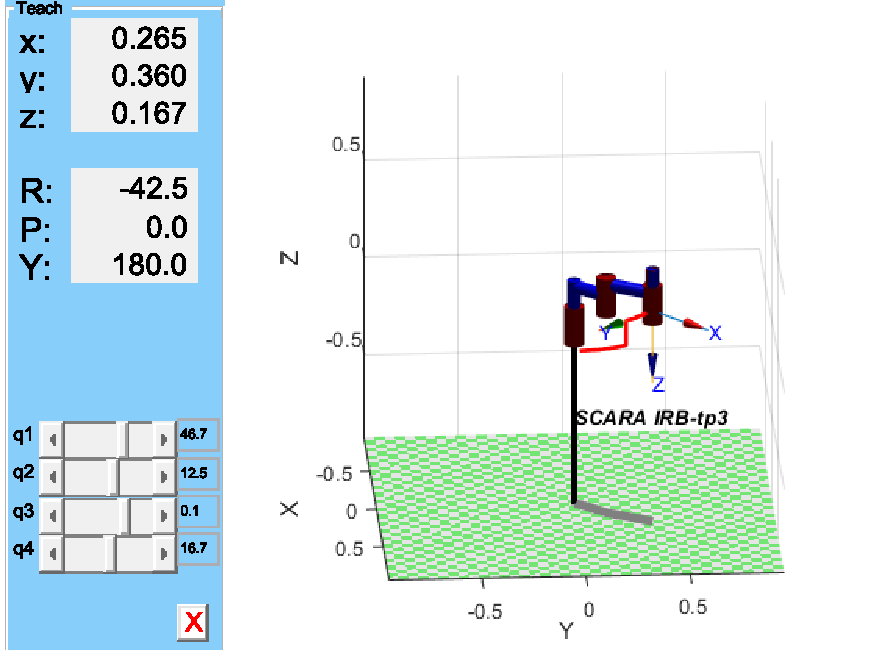
\includegraphics{5-Ejercicio_1_verificacion_Rtp3_teach.pdf}}
    \end{adjustbox}
    \caption{teach Robot tp3}
\end{figure}

\begin{figure}[H]
    \centering
    \begin{adjustbox}{scale = 0.85, max width=\columnwidth}
        \framebox{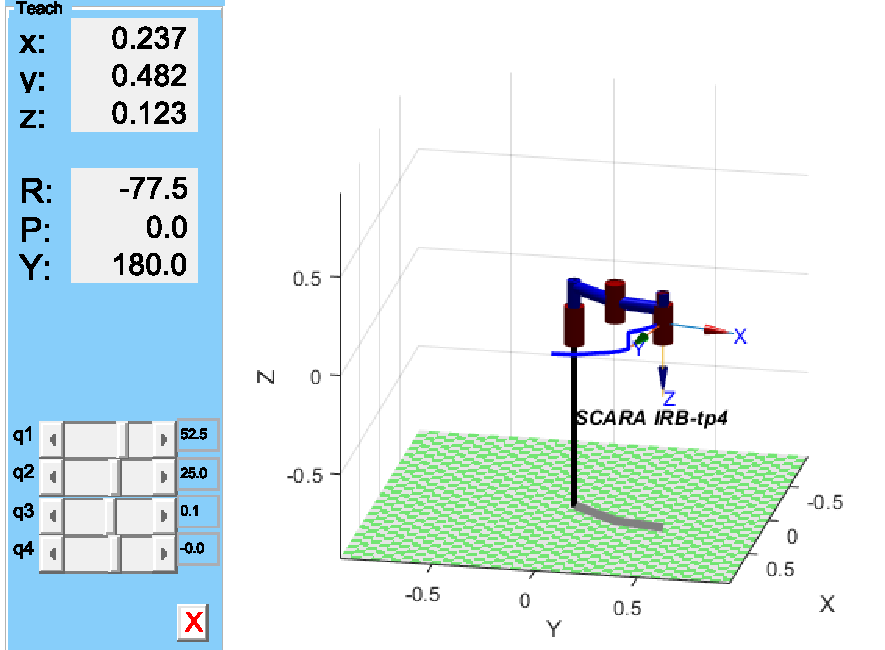
\includegraphics{6-Ejercicio_1_verificacion_Rtp4_teach.pdf}}
    \end{adjustbox}
    \caption{teach Robot tp4}
\end{figure}

\subsection{Comparación de la cinemática directa.}
Cinemática directa de la definición en el TP3: 
\[\left(\begin{array}{cccc} 1.0 & 0 & 0 & 0.45\\ 0 & -1.0 & 0 & 0\\ 0 & 0 & -1.0 & 0.221\\ 0 & 0 & 0 & 1.0 \end{array}\right)\]

Cinemática directa de la definición en el TP4: 
\[\left(\begin{array}{cccc} 1.0 & 0 & 0 & 0.55\\ 0 & -1.0 & 0 & 0\\ 0 & 0 & -1.0 & 0.195\\ 0 & 0 & 0 & 1.0 \end{array}\right)\]

Las diferencias que se presentan en las matrices de cinemática directa es
debido a las razones mencionadas en \cref{subsec: verificacion}, como se puede ver
la diferencia está en el vector de traslación, debido a que se tomaron distintas distancias y al ser modelos de
robot distintos los alcances también lo son. Se ve en cambio que las orientaciones de los sistemas
transformados sí coinciden.

\subsection{}
Todos los resultados se validaron con el método $fkine$ de los robots.

\section{Ejercicio 3}
\subsection{}
\textbf{¿En cuál de las 4 posturas el eje Z del extremo es paralelo al eje Z de la base?}

En la postura dada por la $\mathbf{\overline{q}_1}$. Se puede observar en \cref{T_q1}
que la tercera columna de la matriz de transformación (eje Z del extremo) es un vector
paralelo al eje Z del sistema de la base.

\subsection{}
\textbf{¿En cuál de las 4 posturas el extremo se encuentra más cerca de la base?}

Se puede determinar comparando las normas euclideas de los vectores de traslación (cuarta columna de la matriz de transformación).
La menor de las normas corresponde al sistema con el origen más cercano al sistema de la base.

\begin{table}[H]
    \centering
    \begin{tabular}{|c|c|}
    \hline
    vector & norma (m)      \\ \hline
    $q_1$  & $0.4662$   \\ \hline
    $q_2$  & $0.9182$   \\ \hline
    $q_3$  & $0.9482$   \\ \hline
    $q_4$  & $0.6245$   \\ \hline
    \end{tabular}
    \caption{Distancias al origen del sistema base.}
    \label{normas}
\end{table}

Como se puede ver en la \cref{normas}, la postura dada por $\mathbf{\overline{q}_1}$ es la mas cercana a la base.

\subsection{}
\textbf{¿En cuál de las 4 posturas el eslabón final está orientado en la dirección del eje “Y” de
la base?}

En la postura dada por $\mathbf{\overline{q_3}}$ el eje Z del extremo (en la dirección del eslabón final)
está alineado con el eje Y de la base. Se puede observar en la \cref{T_q3} que la columna
3 (eje Z del extremo) es un vector alineado con el eje Y de la base.

\subsection{}
\textbf{¿En cuál de las 4 posturas el extremo no se encuentra en el primer cuadrante del
sistema de la base?}

Se determina observando las coordenadas del vector de traslación de las matrices de transformación homogénea (cuarta columna).
\begin{itemize}
    \item Visto en el plano XY, la postura dada por $\mathbf{\overline{q_1}}$ no cae estrictamente en el primer cuadrante sino sobre el eje X de la base.
    \item Visto en el plano XY, la postura dada por $\mathbf{\overline{q_4}}$ no cae en el primer cuadrante.
    \item Visto en el plano XZ, ninguna postura cae fuera del primer cuadrante.
    \item Visto en el plano YZ, la postura dada por $\mathbf{\overline{q_4}}$ no cae en el primer cuadrante.
    \item Visto en el plano YZ, la postura dada por $\mathbf{\overline{q_1}}$ no cae estrictamente en el primer cuadrante sino sobre el eje Z de la base.
\end{itemize}

\subsection{}
\textbf{¿Qué condición debe cumplirse en la matriz homogénea total del robot para que los
ejes del sistema del extremo sean paralelos (sin importar orientación ni orden) a los
del sistema de la base?}

En la sub-matriz de rotación debe habe a lo sumo un 1 o -1 en cada columna y estos encontrarse en distintas filas, esto hace que los ejes del sistema del extremo sean paralelos a los ejes del sistema de la base (en igual sentido o en el opuesto)
y que además no sean vectores paralelos entre sí.
Además el determinante de esta sub-matriz debe ser 1 y no -1 (esto garantiza que sea un sistema dextrógiro).

\subsection{}
\textbf{¿Por qué las siguientes matrices no pueden ser resultado de ningún vector de
posiciones articulares?}

La siguiente no puede ser una matriz de transformación homogénea dado que,
como se puede observar en la sub-matriz de rotación, los vectores en la columna 1 y 3 son paralelos entre sí 
y por lo tanto, esta matriz \textbf{no determina un sistema de referencia ortonormal}.

\begin{equation*}
    T = 
    \begin{bmatrix}
        0 & 1 & 0 & 0.3946\\
        0 & 0 & 0 & 0.2947\\
        1 & 0 & 1 & 0.8103\\
        0 & 0 & 0 & 1     \\
    \end{bmatrix}
\end{equation*}

La siguiente no puede ser matriz de transformación para este robot dado ya que \textbf{se exceden
los límites del espacio de trabajo alcanzable por el extremo del robot}. Cómo se puede observar en la
\cref{alcance fanuc}, el máximo alcance radial es de $0.704\,m$ mientras que la distancia respecto del sistema base,
solo en el plano XY (dado por la norma en el plano XY del vector de traslación), es de $2.12\,m$.

\begin{equation*}
    T = 
    \begin{bmatrix}
        0.7071  &  0  & 0.7071 & 1.4971\\
        -0.7071 &  0  & 0.7071 & 1.4971\\
        1       & -1  &    0   & 0.5250\\
        0       &  0  &    0   &    1  \\
    \end{bmatrix}
\end{equation*}

\begin{figure}[H]
    \centering
    \begin{adjustbox}{scale = 0.65, max width=\columnwidth}
        \framebox{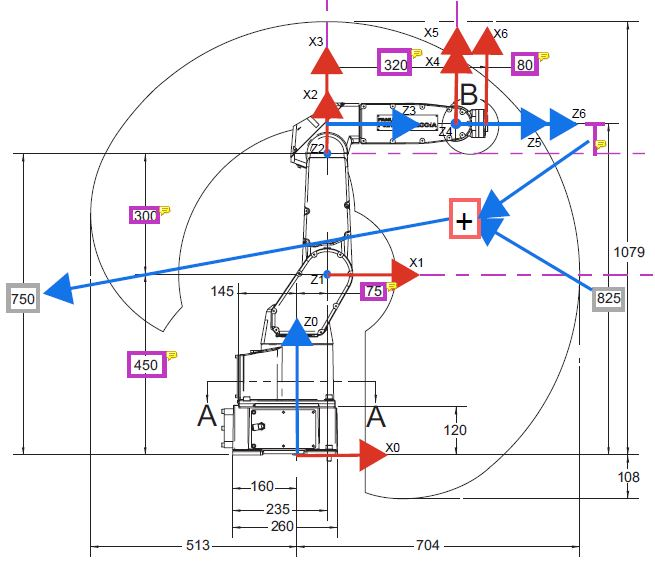
\includegraphics{7-Fanuc_alcance.JPG}}
    \end{adjustbox}
    \caption{Vista lateral FANUC.}
    \label{alcance fanuc}
\end{figure}

La siguiente no es una matriz de transformación para este robot dado que también \textbf{se exceden
los límites del espacio de trabajo alcanzable por el extremo del robot}. En este caso no es tan evidente como en el caso anterior,
asi que en las \cref{teach fanuc alcance vista} y \cref{teach fanuc alcance lateral} se muestra una trayectoria del robot a lo largo de su límite del espacio de trabajo en comparación con la posición
esperada según la matriz de transformación.

\begin{equation*}
    T = 
    \begin{bmatrix}
        0  &  0   & 1 & 0      \\
        0  &  -1  & 0 & 0.7030 \\
        1  &  0   & 0 & 0      \\
        0  &  0   & 0 & 1      \\
    \end{bmatrix}
\end{equation*}

\begin{figure}[H]
    \centering
    \begin{adjustbox}{scale = 0.8, max width=\columnwidth}
        \framebox{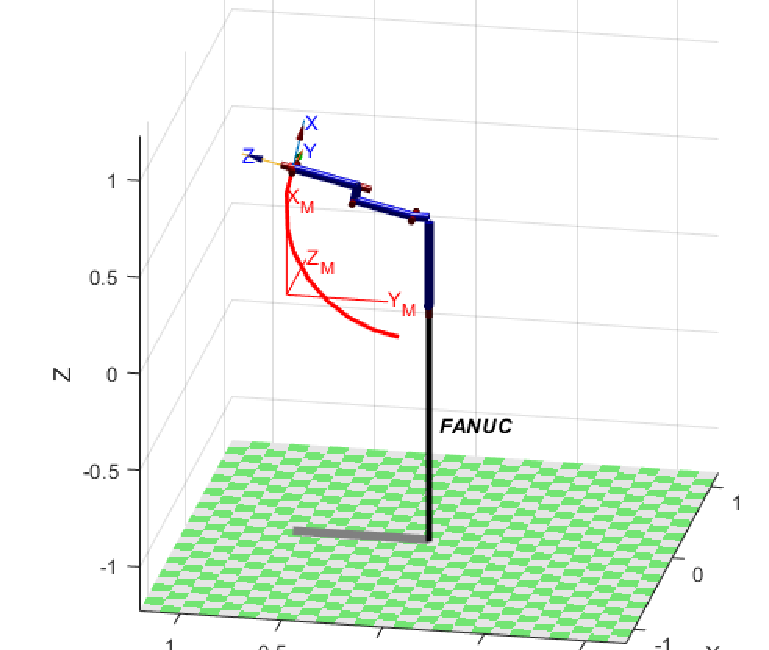
\includegraphics{8-Ejercicio_3_6_T2_1.pdf}}
    \end{adjustbox}
    \caption{Vista alcance FANUC}
    \label{teach fanuc alcance vista}
\end{figure}

\begin{figure}[H]
    \centering
    \begin{adjustbox}{scale = 0.8, max width=\columnwidth}
        \framebox{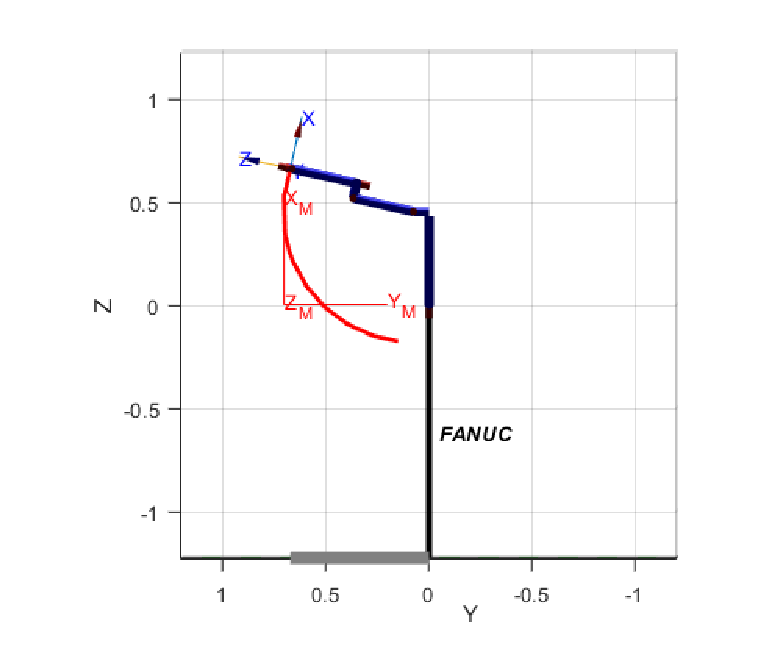
\includegraphics{9-Ejercicio_3_6_T2_2.pdf}}
    \end{adjustbox}
    \caption{Vista lateral alcance FANUC.}
    \label{teach fanuc alcance lateral}
\end{figure}

Para verificar la siguiente matriz, nuevamente se hace uso del robotic toolbox
para tratar de alcanzar la postura dada haciendo uso del método teach del robot.
Como se puede ver en la \cref{verificacion T1}, a priori (no puedo saber con total exactitud),
\textbf{el extremo del robot sí puede alcanzar la postura dada}.

\begin{equation*}
    T = 
    \begin{bmatrix}
        0  &  0.500   & 0.866 & 0.4971   \\
        0  &  -0.866  & 0.500 & 0.4971   \\
        1  &  0.000   & 0.000 & 0.5250   \\
        0  &  0       & 0     & 1        \\
    \end{bmatrix}
\end{equation*}

\begin{figure}[H]
    \centering
    \begin{adjustbox}{max width=\columnwidth}
        \framebox{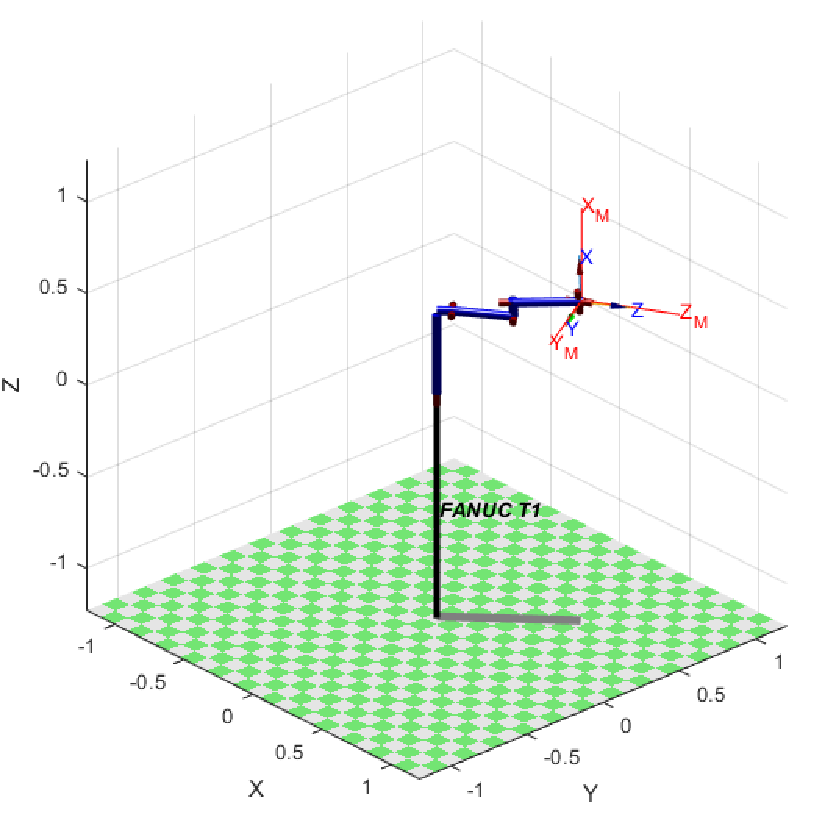
\includegraphics{10-Ejercicio_3_6_T1.pdf}}
    \end{adjustbox}
    \caption{Verificación de la postura dada por T1}
    \label{verificacion T1}
\end{figure}

\section{Ejercicio 4}
\textbf{Calcule el máximo error de posición cartesiana en el extremo final
que podría tener el LBR iiwa 7 R800 (KUKA). Para hacerlo, asuma que está en
una postura totalmente vertical y extendida, y que todas sus articulaciones
tienen un error de posición (delta de posición) de 0,1º}

\subsection{}
\textbf{¿Cuál es el error en esta situación?}

Se elaboró un código para determinar el error.
Por un lado se calcula la cinemática directa del robot con las coordenadas articulares exactas correspondientes
a la posición vertical y luego se calcula la cinemática directa sumando a dicho vector de coordenadas
un error de 0.1° (positivo) en todas las articulaciones, con el objeto de obtener el maximo error.
El error de posicionamiento se obtiene como la norma de la diferencia entre los vectores de traslación de las dos transformaciones.
El error que se obtiene es de $\mathbf{2.1468 mm}$.

\subsection{}
\textbf{¿El error es el mismo para cualquier posición? (suponiendo constante el error de
posición articular).}

A priori se puede decir que el error de posicionamiento no será el mismo para distintas posturas
dado que el mismo error en las sucesivas variables articulares tendrá un efecto
distinto en el error cartesiano dependiendo de cuál sea la postura.

Se elabora un contraejemplo con otra posición articular genérica y, como en el caso anterior, se obtiene el error de posicionamiento.
En este caso el error es de $\mathbf{2.0611 mm}$.

\subsection{}
\textbf{¿La respuesta anterior es válida para todo tipo de robots serie?}

En principio sí.

\section{Ejercicio TF}
A continuación, se pueden ver curvas características del espacio de trabajo en el plano XY y XZ.
Luego, puede visualizarse una imagen obtenida de Internet (\href{https://www.universal-robots.com/articles/ur/release-notes/release-note-software-version-512xx/}{espacio de trabajo}) en la cual se
observa el espacio de trabajo total, lo que se coincide con nuestra estimación.

\begin{figure}[H]
    \centering
    \begin{adjustbox}{max width=\columnwidth}
        \framebox{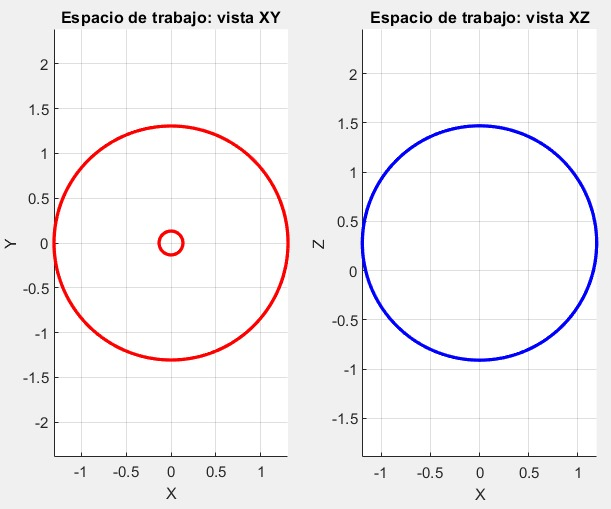
\includegraphics{13-Curvas_esp_trabajo.jpeg}}
    \end{adjustbox}
    \caption{Curvas del espacio de trabajo otenidas}
\end{figure}

\begin{figure}[H]
    \centering
    \begin{adjustbox}{max width=\columnwidth}
        \framebox{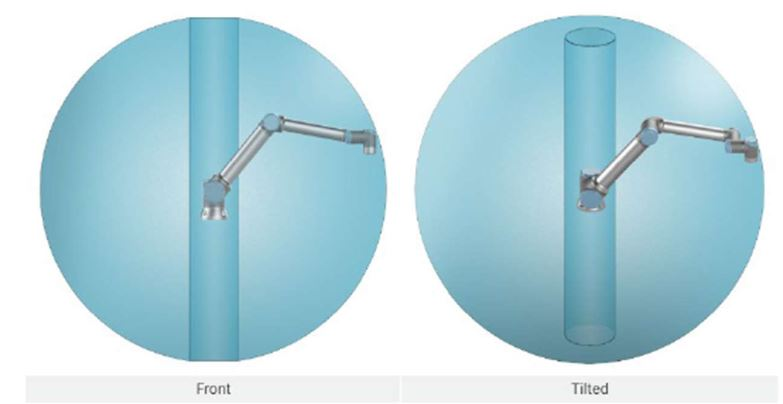
\includegraphics{14-Curvas_esp_trabajo_internet.JPG}}
    \end{adjustbox}
    \caption{Espacio de trabajo obtenido en internet.}
\end{figure}

De acuerdo con la matriz de base, la misma está definida en robot.m y corresponde a una
fundación de 0.1m de altura.
Aún no contamos con las dimensiones del gripper para poder asignar una dimensión, pero se
definió una variable ``distancia\_TC'' genérica que corresponde a la distancia que se trasladará
el TCP (Tool Center Point) desde el origen del último sistema y en base a esta también se definió
la matriz de ``tool''.

%\begin{equation*}
%    \prescript{O}{}{Rot_M} = 
%    \begin{bmatrix}
%        0.500 & -0.866\\
%        0.866 & 0.500
%    \end{bmatrix}
%\end{equation*}

%\begin{figure}[H]
%    \centering
%    \begin{adjustbox}{scale = 0.85, max width=\columnwidth}
%        \framebox{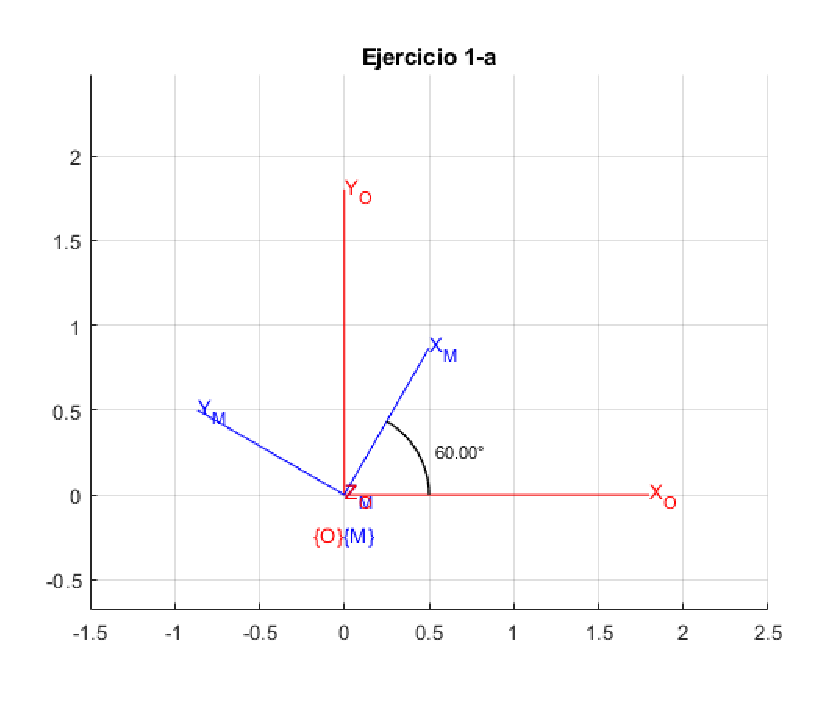
\includegraphics{1-Ejercicio_1_a.pdf}}
%    \end{adjustbox}
%    \caption{Sistema O y Sistema M superpuestos con indicación de ángulo de rotación.}
%\end{figure}


%\begin{table}[H]
%    \centering
%    \begin{tabular}{|c|c|c|c|c|c|}
%    \hline
%    Sistema & $\theta$  & $d$           & $a$    & $\alpha$ & $\sigma$ \\ \hline
%    1       & $q_1$     & $199.2$       & $200$  & 0        & 0        \\ \hline
%    2       & $q_2$     & $59.5$        & $250$  & 0        & 0        \\ \hline
%    3       & $0$       & $q_3$         & $0$    & 180°     & 1        \\ \hline
%    4       & $q_4$     & $37.5$        & $0$    & 0        & 0        \\ \hline
%    \end{tabular}
%    \caption{Parámetros DH alternativos.}
%    \label{parametros DH2}
%\end{table}

\end{document}